
\subsection{Shape Initialization}
\label{sec:initialization}


Initially, we assume that the 2D layout $\mathcal{L}$ lies on the $XOY$ plane, so that each vertex $\mathbf{v}_i(x_i,y_i,z_i)$ in $V$ has $z_i=0$. 
Each panel in $P$ has a normal $\mathbf{n}_i=(0,0,1)^T$. 
To construct the 3D model, we can compute the 3D coordinates of all the vertexes. 
%
When humans fold a carton, the general process begins by folding each edge at a rough angle and then connecting the closest vertexes to obtain a box-like shape. 
%
Instead of directly computing the vertex coordinates, it is natural to first fold the 2D layout by assigning a rotation angle to each pair of adjacent panels in order to obtain a rough shape.
%
As seen in existing designs on the Internet, most of the traditional cartons are cuboid for the purpose of holding files or delivering daily supplies. 
Although there is a recent trend to design more complicated layouts to attract consumers, the shape of these unusual cartons is similar to traditional boxes, as their functions are still packaging commodities. 
%
Therefore, we choose $\pi/2$ as the initial value of the rotation angle at each folding edge. 
%
First, a panel graph of a layout is constructed, as shown in Figure~\ref{fig:midresult} (a).
Each panel is a node, and there is an edge between two panels if they are connected by a folding edge.
%
All panels in the 2D layout are recursively folded in a breadth-first manner.
Starting from the panel with the maximal area, our system folds all of its adjacent panels by rotating them around their connecting edge by $\pi/2$ and then continuing to the others. 
Figure~\ref{fig:midresult} illustrates the folding process of a cuboid carton. 

\begin{figure}
	\centering
	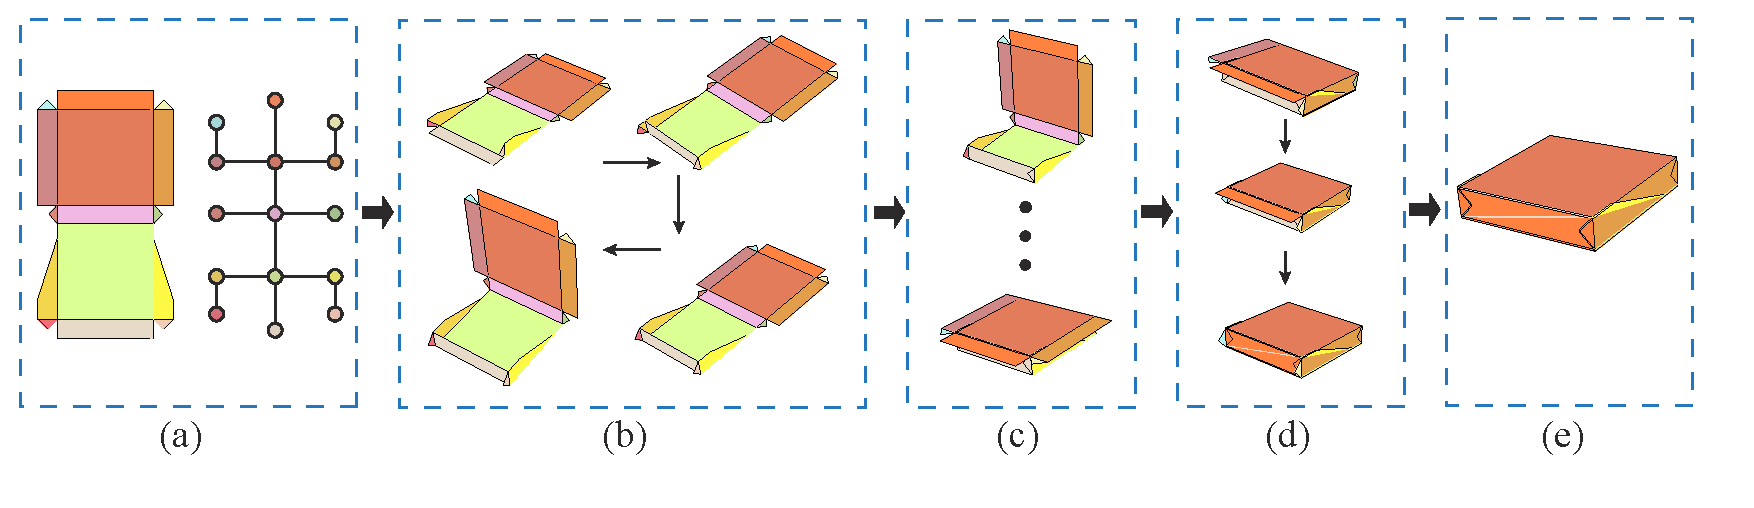
\includegraphics[width=0.9\textwidth]{images/midresult}
	\caption{A rough 3D shape is obtained by folding the edges between adjacent panels by $\pi/2$ in the 2D layout (a). This is carried out in a breadth-first manner, starting from the panel with the maximal area. (b), (c), (d) and (e) are the different folding stages in the initialization step.}
	\label{fig:midresult}
\end{figure}



Traditional cartons in cuboid shapes can reach an ideal state.
Figure~\ref{fig:initial-automatic} shows a group of results that are generated by simply folding adjacent panels by $\pi/2$.
%
However, many complicated designs still need refinement, such as the four examples in Figure~\ref{fig:initial-need-improvement}. 
If we take the hexagonal box as an example, the 3D model can be improved by simply snapping the small glue flaps to their nearby side panels to ensure that the carton is stable without any manual intervention. 
In most cases, it is common practice to attach a glued flap to a side panel in order to assemble a closed box.
%
As a result, we develop a suggestive interface that automatically detects potential geometric modifications from the rough carton shape and provides these suggestions for users to explore.

\begin{figure}
	\centering
	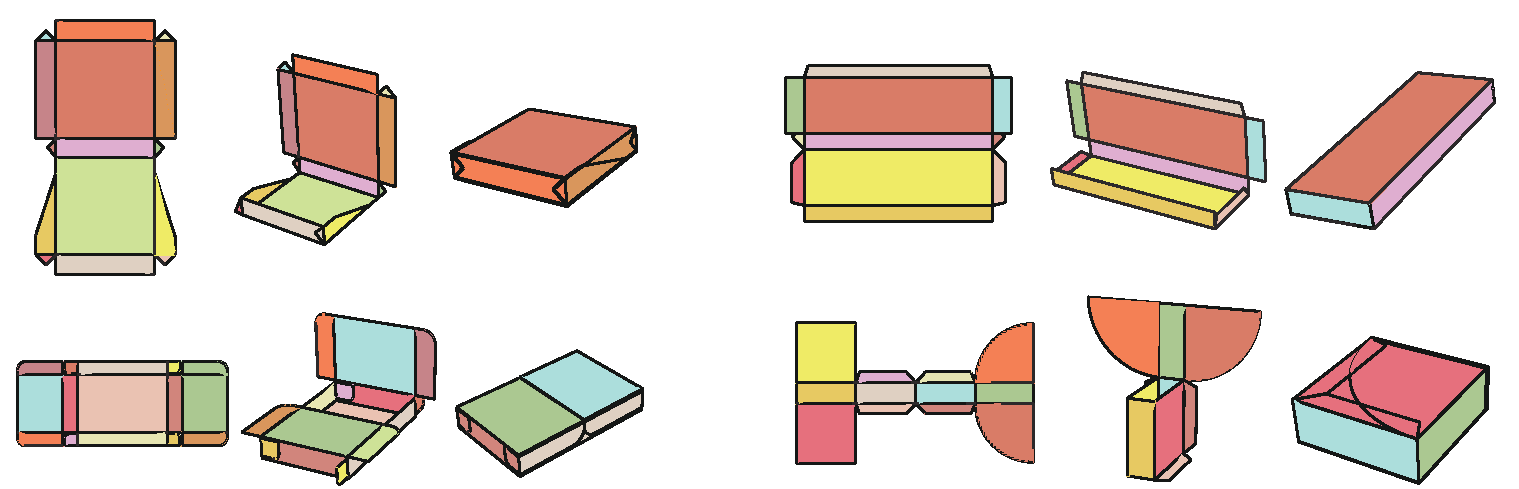
\includegraphics[width=0.8\textwidth]{images/initiala}
	\caption{Four examples of carton models that can be fully automatically generated from 2D layouts by folding each edge at a fixed angle $\pi/2$. }
	\label{fig:initial-automatic}
\end{figure}

 
\begin{figure}
	\centering
	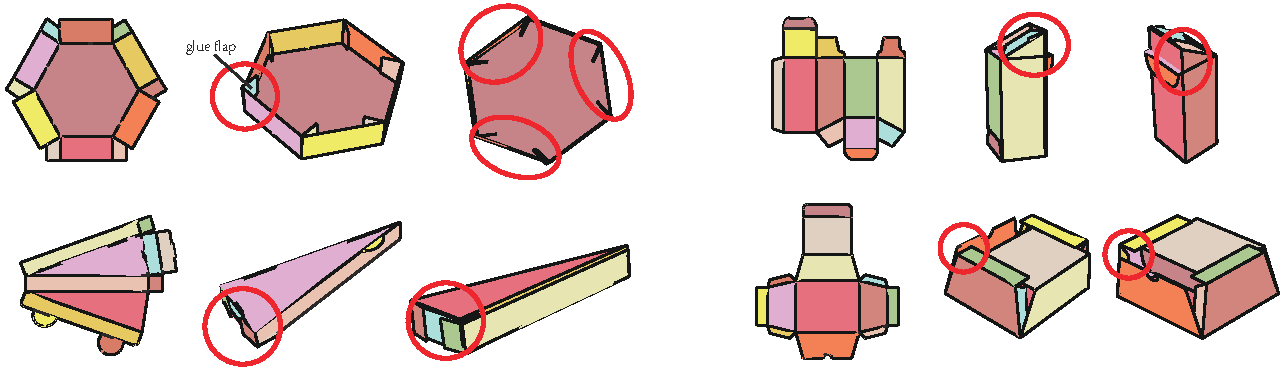
\includegraphics[width=0.8\textwidth]{images/initialb}
	\caption{Four examples of the carton models that need more shape improvement. While the shapes are not cuboid, using a fixed angle $\pi/2$ leads to non-closed shapes and loose structures.}
	\label{fig:initial-need-improvement}
\end{figure}
%%%%%%%%%%%%%%%%%%%%%%%%%%%%%%%%%%%%%%%%%%%%%%%%%%%%%%%%%%%%%%%%%%%%%
